\documentclass[10pt]{article}
\usepackage{xr}

\usepackage{graphicx}
\usepackage{amsfonts}
\usepackage{pifont}
\newcommand{\cmark}{\ding{51}}%
\newcommand{\xmark}{\ding{55}}%

\linespread{1}
\addtolength{\oddsidemargin}{-2.5cm}
%\addtolength{\evensidemargin}{-3cm}
\addtolength{\textwidth}{2.5cm}

\setcounter{figure}{2}    
\begin{document}




\begin{figure}
\caption{Genome-wide association mapping results from the analysis of the mouse data for the single-locus method FaST-LMM and the 
multiple-locus method
Eagle. Eagle was run under two settings; its default setting (Eagle$^{default}$) and where the model selection criterion had been optimised 
for a false discovery rate of 5\% (Eagle$^{optimal}$). 
The number of SNP-trait associations found are reported. The bar plots with boxes around them are for those traits where using 
Eagle$^{default}$ and Eagle$^{optimal}$ resulted in more findings than with single-locus analysis.} 
\label{figmouse}
\begin{center}
%% obtained from bracewell by running ResultsV2.R from /data/geo047/MWAM/Mouse/OutBred/RScripts/
\includegraphics[width=15cm, height=15cm]{mouseresults.eps}
\end{center}

\end{figure}






\end{document}
